\documentclass[]{article}
\usepackage{lmodern}
\usepackage{amssymb,amsmath}
\usepackage{ifxetex,ifluatex}
\usepackage{fixltx2e} % provides \textsubscript
\ifnum 0\ifxetex 1\fi\ifluatex 1\fi=0 % if pdftex
  \usepackage[T1]{fontenc}
  \usepackage[utf8]{inputenc}
\else % if luatex or xelatex
  \ifxetex
    \usepackage{mathspec}
  \else
    \usepackage{fontspec}
  \fi
  \defaultfontfeatures{Ligatures=TeX,Scale=MatchLowercase}
\fi
% use upquote if available, for straight quotes in verbatim environments
\IfFileExists{upquote.sty}{\usepackage{upquote}}{}
% use microtype if available
\IfFileExists{microtype.sty}{%
\usepackage{microtype}
\UseMicrotypeSet[protrusion]{basicmath} % disable protrusion for tt fonts
}{}
\usepackage[margin=1in]{geometry}
\usepackage{hyperref}
\hypersetup{unicode=true,
            pdftitle={Lab 1 - Gr. 14 - Bioinformatics (732A93)},
            pdfauthor={tbd},
            pdfborder={0 0 0},
            breaklinks=true}
\urlstyle{same}  % don't use monospace font for urls
\usepackage{color}
\usepackage{fancyvrb}
\newcommand{\VerbBar}{|}
\newcommand{\VERB}{\Verb[commandchars=\\\{\}]}
\DefineVerbatimEnvironment{Highlighting}{Verbatim}{commandchars=\\\{\}}
% Add ',fontsize=\small' for more characters per line
\usepackage{framed}
\definecolor{shadecolor}{RGB}{248,248,248}
\newenvironment{Shaded}{\begin{snugshade}}{\end{snugshade}}
\newcommand{\KeywordTok}[1]{\textcolor[rgb]{0.13,0.29,0.53}{\textbf{#1}}}
\newcommand{\DataTypeTok}[1]{\textcolor[rgb]{0.13,0.29,0.53}{#1}}
\newcommand{\DecValTok}[1]{\textcolor[rgb]{0.00,0.00,0.81}{#1}}
\newcommand{\BaseNTok}[1]{\textcolor[rgb]{0.00,0.00,0.81}{#1}}
\newcommand{\FloatTok}[1]{\textcolor[rgb]{0.00,0.00,0.81}{#1}}
\newcommand{\ConstantTok}[1]{\textcolor[rgb]{0.00,0.00,0.00}{#1}}
\newcommand{\CharTok}[1]{\textcolor[rgb]{0.31,0.60,0.02}{#1}}
\newcommand{\SpecialCharTok}[1]{\textcolor[rgb]{0.00,0.00,0.00}{#1}}
\newcommand{\StringTok}[1]{\textcolor[rgb]{0.31,0.60,0.02}{#1}}
\newcommand{\VerbatimStringTok}[1]{\textcolor[rgb]{0.31,0.60,0.02}{#1}}
\newcommand{\SpecialStringTok}[1]{\textcolor[rgb]{0.31,0.60,0.02}{#1}}
\newcommand{\ImportTok}[1]{#1}
\newcommand{\CommentTok}[1]{\textcolor[rgb]{0.56,0.35,0.01}{\textit{#1}}}
\newcommand{\DocumentationTok}[1]{\textcolor[rgb]{0.56,0.35,0.01}{\textbf{\textit{#1}}}}
\newcommand{\AnnotationTok}[1]{\textcolor[rgb]{0.56,0.35,0.01}{\textbf{\textit{#1}}}}
\newcommand{\CommentVarTok}[1]{\textcolor[rgb]{0.56,0.35,0.01}{\textbf{\textit{#1}}}}
\newcommand{\OtherTok}[1]{\textcolor[rgb]{0.56,0.35,0.01}{#1}}
\newcommand{\FunctionTok}[1]{\textcolor[rgb]{0.00,0.00,0.00}{#1}}
\newcommand{\VariableTok}[1]{\textcolor[rgb]{0.00,0.00,0.00}{#1}}
\newcommand{\ControlFlowTok}[1]{\textcolor[rgb]{0.13,0.29,0.53}{\textbf{#1}}}
\newcommand{\OperatorTok}[1]{\textcolor[rgb]{0.81,0.36,0.00}{\textbf{#1}}}
\newcommand{\BuiltInTok}[1]{#1}
\newcommand{\ExtensionTok}[1]{#1}
\newcommand{\PreprocessorTok}[1]{\textcolor[rgb]{0.56,0.35,0.01}{\textit{#1}}}
\newcommand{\AttributeTok}[1]{\textcolor[rgb]{0.77,0.63,0.00}{#1}}
\newcommand{\RegionMarkerTok}[1]{#1}
\newcommand{\InformationTok}[1]{\textcolor[rgb]{0.56,0.35,0.01}{\textbf{\textit{#1}}}}
\newcommand{\WarningTok}[1]{\textcolor[rgb]{0.56,0.35,0.01}{\textbf{\textit{#1}}}}
\newcommand{\AlertTok}[1]{\textcolor[rgb]{0.94,0.16,0.16}{#1}}
\newcommand{\ErrorTok}[1]{\textcolor[rgb]{0.64,0.00,0.00}{\textbf{#1}}}
\newcommand{\NormalTok}[1]{#1}
\usepackage{graphicx,grffile}
\makeatletter
\def\maxwidth{\ifdim\Gin@nat@width>\linewidth\linewidth\else\Gin@nat@width\fi}
\def\maxheight{\ifdim\Gin@nat@height>\textheight\textheight\else\Gin@nat@height\fi}
\makeatother
% Scale images if necessary, so that they will not overflow the page
% margins by default, and it is still possible to overwrite the defaults
% using explicit options in \includegraphics[width, height, ...]{}
\setkeys{Gin}{width=\maxwidth,height=\maxheight,keepaspectratio}
\IfFileExists{parskip.sty}{%
\usepackage{parskip}
}{% else
\setlength{\parindent}{0pt}
\setlength{\parskip}{6pt plus 2pt minus 1pt}
}
\setlength{\emergencystretch}{3em}  % prevent overfull lines
\providecommand{\tightlist}{%
  \setlength{\itemsep}{0pt}\setlength{\parskip}{0pt}}
\setcounter{secnumdepth}{0}
% Redefines (sub)paragraphs to behave more like sections
\ifx\paragraph\undefined\else
\let\oldparagraph\paragraph
\renewcommand{\paragraph}[1]{\oldparagraph{#1}\mbox{}}
\fi
\ifx\subparagraph\undefined\else
\let\oldsubparagraph\subparagraph
\renewcommand{\subparagraph}[1]{\oldsubparagraph{#1}\mbox{}}
\fi

%%% Use protect on footnotes to avoid problems with footnotes in titles
\let\rmarkdownfootnote\footnote%
\def\footnote{\protect\rmarkdownfootnote}

%%% Change title format to be more compact
\usepackage{titling}

% Create subtitle command for use in maketitle
\newcommand{\subtitle}[1]{
  \posttitle{
    \begin{center}\large#1\end{center}
    }
}

\setlength{\droptitle}{-2em}

  \title{Lab 1 - Gr. 14 - Bioinformatics (732A93)}
    \pretitle{\vspace{\droptitle}\centering\huge}
  \posttitle{\par}
    \author{tbd}
    \preauthor{\centering\large\emph}
  \postauthor{\par}
    \date{}
    \predate{}\postdate{}
  
\usepackage{booktabs}
\usepackage{longtable}
\usepackage{array}
\usepackage{multirow}
\usepackage[table]{xcolor}
\usepackage{wrapfig}
\usepackage{float}
\usepackage{colortbl}
\usepackage{pdflscape}
\usepackage{tabu}
\usepackage{threeparttable}
\usepackage{threeparttablex}
\usepackage[normalem]{ulem}
\usepackage{makecell}

\begin{document}
\maketitle

\section{Assignment 1}\label{assignment-1}

\section{Question 1: Hardyâ€``Weinberg equilibrium \#\# Question
1.1}\label{question-1-hardyaweinberg-equilibrium-question-1.1}

We define the following probability space

\[\left(\Omega,\mathcal{F},P\right)\]

Where,

\[\Omega = \left\{(A,A), (A,a), (a,A), (a,a)\right\}\]

We also define a probability measure \(P\) such as

\[P(X, Y)\] \[X,Y \in \left\{A, a\right\}\]

So \(P(X,Y)\) is the probability that an allele is \((X,Y)\).

By definition, \(p\) is the proportion of \(A's\) in the allele
population and \(q\) is the proportion of \(a's\) in the allele
population, so:

\[P(A) = P(A,A) + P(A,a) + P(a,A) = p\]

The same applies to \(P(a)\). \[P(a) = P(a,a) + P(a,A) + P(A,a)= q\]

The fact that we asume random mating means that \(X\) and \(Y\) are
\(IID\), which entails the following:

\[P(A,A) = P(A) * P(A) = p^{2}\] \[P(a,a) = P(a) * P(a) = q^{2}\]
\[P(A,a) = P(a,A) = P(A)*P(a) = pq\] The probability of an allele of it
being a heterozygote is: \[P(A,a) + P(a,A) = 2pq\]

\[P(\Omega) = P(A,A) + P(a,a) + 2P(A,a) = p^{2} + q^{2} + 2pq = 1\]

Thus, we show that by random mating the proportion of \(A's\) and
\(a's\) is the same in the offsprings and the Hardy-Weinberg equilibrium
is obtained and can't deviate from it.

\subsection{Question 1.2}\label{question-1.2}

We now look at the MN blood group, that has two possible
coâ€``dominating alleles, \(L^{M}\) (denoted \(M\)) and \(L^{N}\)
(denoted \(N\)). In a population of \(n = 1000\) Americans of Caucasian
descent, the following genotype counts were observed:

\begin{itemize}
\item
  \(n_{MM} = 357\) individuals were \emph{MM} homozygotes;
\item
  \(n_{MN} = 485\) individuals were \emph{MN} heterozygotes;
\item
  \(n_{NN} = 158\) individuals were \emph{NN} homozygotes;
\end{itemize}

The relatives proportion, obtained by dividing the genotype counts by
the total population, are 0.357, 0.485 and 0.158 respectively. According
to the Hardyâ€``Weinberg principle, we expect these quantities to follow
the proportions \(p^2\), \(2pq\) and \(q^2\), where \(p\) and \(q\) are
the proportions of \(N\) and \(M\) in the alleles. In formulas:

\begin{equation}
  \begin{split}
    p & = \frac{n_{MM}}{n} + \frac{1}{2} \cdot \frac{n_{MN}}{n} = 0.357 + \frac{1}{2} \cdot 0.485 = 0.5995 \\
    q & = \frac{n_{NN}}{n} + \frac{1}{2} \cdot \frac{n_{MN}}{n} = 0.158 + \frac{1}{2} \cdot 0.485 = 0.4005 
  \end{split}
\end{equation}

With these empirical quantities we formulate what would the population
look if it was on equilibrium and compare them with the real proportions
\(\left(p_{MM}=0.375, p_{NN}=0.158, p_{MN}=0.485\right)\):

\[p_{MM}^0 = p^{2} = 0.3594002\] \[p_{NN}^0 = q^{2} = 0.1604002\]
\[p_{MN}^0 = 2pq = 0.4801995\]

Performing a chiâ€``square goodness of fit test (\texttt{chisq.test()}
function in R) results in \emph{p-value} \(= 1\). This result shows that
there is not enough statistical evidence to reject the hypothesis that
the population is in a Hardy-Weinberg equilibrium.

\begin{verbatim}
## Warning in chisq.test(c(0.357, 0.485, 0.158), p = c(p_2, pq, q_2)): Chi-
## squared approximation may be incorrect
\end{verbatim}

\begin{verbatim}
## 
##  Chi-squared test for given probabilities
## 
## data:  c(0.357, 0.485, 0.158)
## X-squared = 9.9938e-05, df = 2, p-value = 1
\end{verbatim}

\section{Assignment 2}\label{assignment-2}

Note that, by convention, a \emph{coding strand} is used when displaying
a DNA sequence. ``A coding strand, is the segment within double-stranded
DNA that runs from 5' to 3', and which is complementary to the antisense
strand of DNA, or template strand, which runs from 3' to 5'''
(\url{https://en.wikipedia.org/wiki/Sense_strand}).

\subsection{2.1}\label{section}

We go to the following link
\url{https://www.ncbi.nlm.nih.gov/nuccore/CU329670}, scroll down to
``Features'', click on ``CDS'' to see the first 5662 nucleotides of the
sequence.

The protein product is: \textbf{RecQ type DNA helicase}

\subsection{2.2}\label{section-1}

Note that proteins are made up of 20 different amino acids (linked
together). Amino acids are molecules composed of an alpha carbon, a
carboxyl group, an amino group and a side chain. The side chain is what
makes an amino acid unique (see p.~5, Concepts in Bioinformatics and
Genomics). The 20 different amino acids can be found in the picture
below.

In our case, the first four amino acids are:

\begin{enumerate}
\def\labelenumi{\arabic{enumi}.}
\tightlist
\item
  M (= \textbf{Methionine}, coded by ATG, representing the starting
  sequence)
\item
  V (= \textbf{Valine})
\item
  V (= \textbf{Valine})
\item
  A (= \textbf{Alanine})
\end{enumerate}

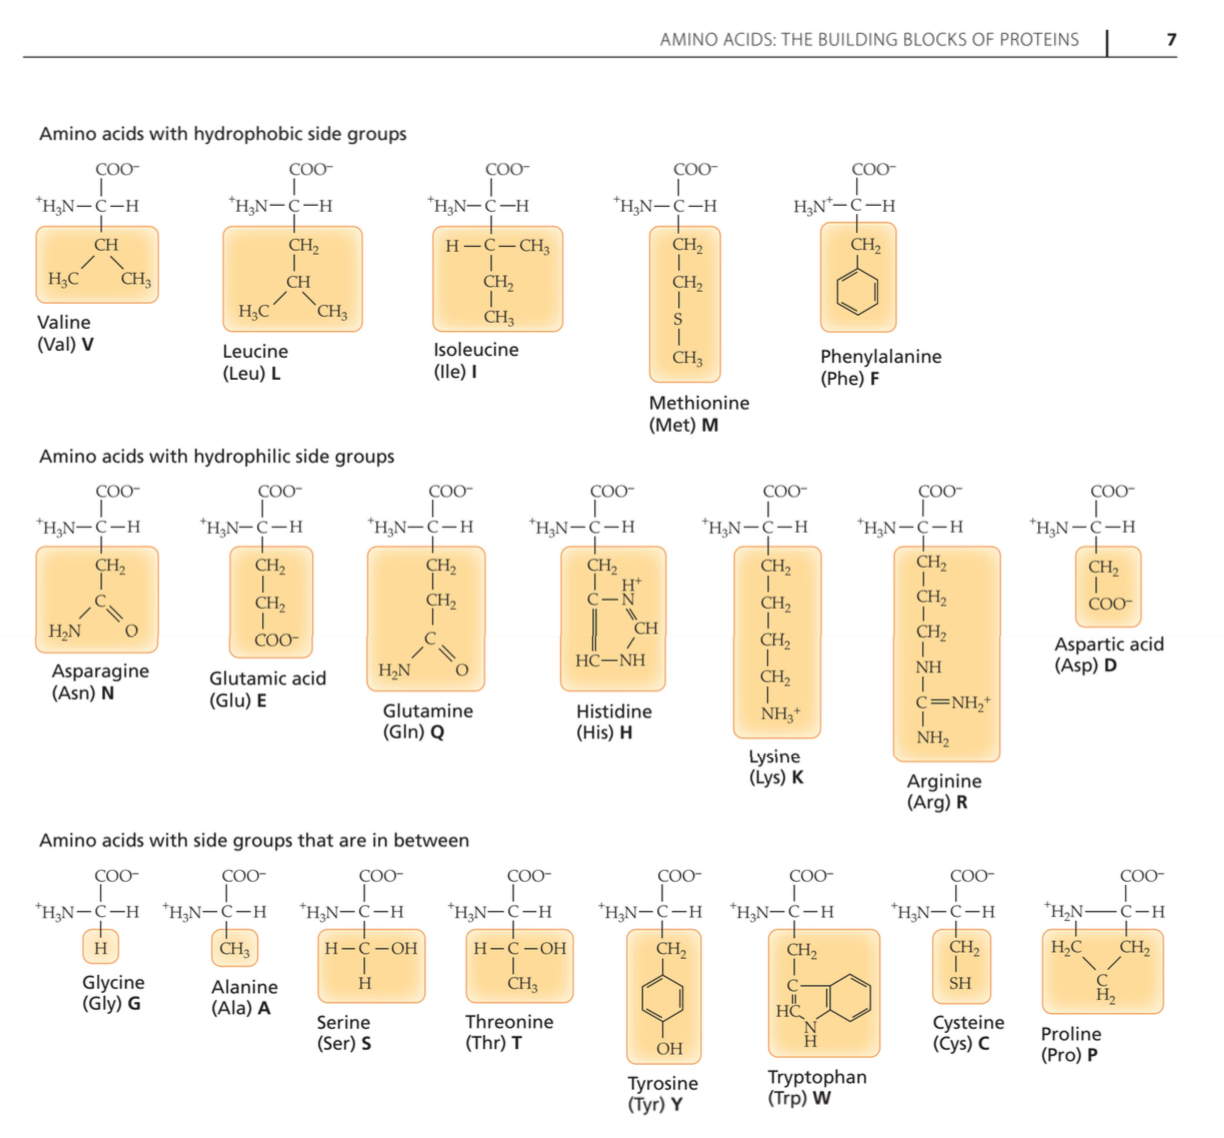
\includegraphics[width=400px]{images/2.2_amino-acids}

\subsection{2.3}\label{section-2}

Note that nucleotides code for amino acids. They are molecules composed
of a sugar, a phosphate and a base. The part of nucleotides that
distinguishes them is the base.

There are four possible bases: A (Adenine), C (Cytosine), G (Guanine), T
(Thymine)

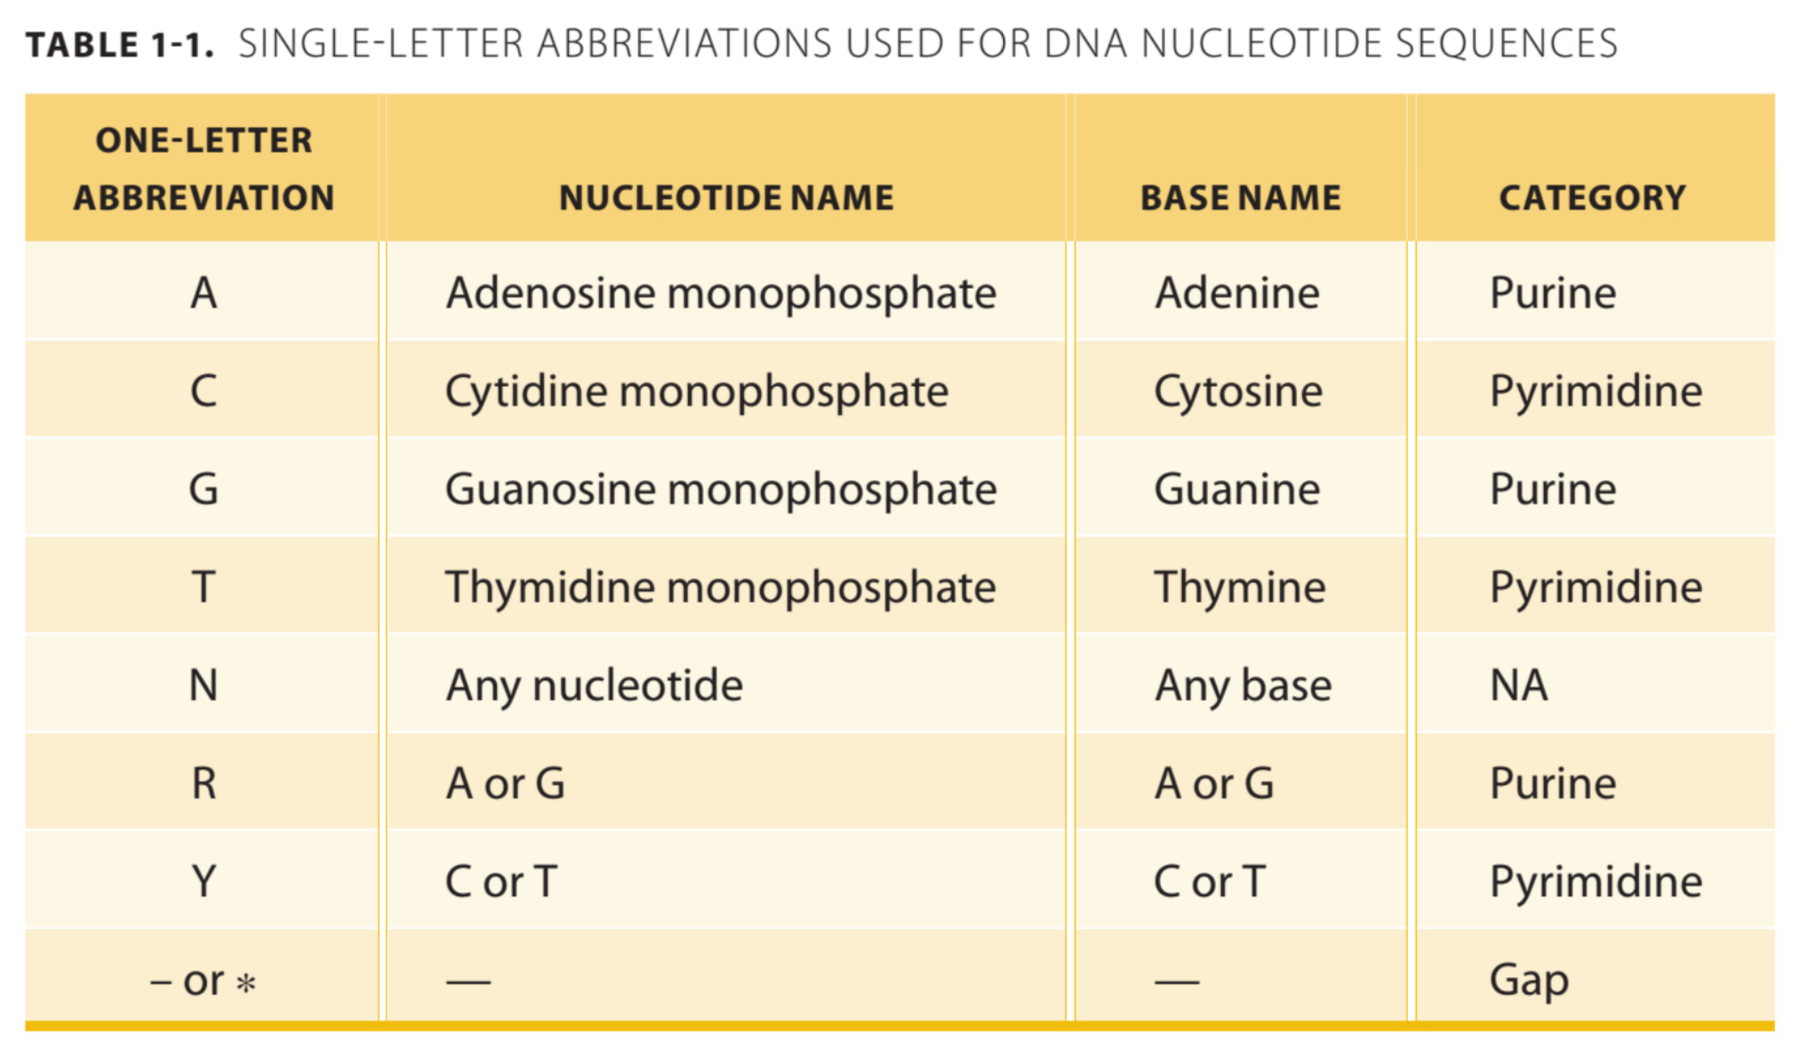
\includegraphics[width=300px]{images/2.3_nucleotides}

Specific combinations of these nucleotides code for specific amino
acids. In genetic code, three nucleotides (called codon) always code for
one amino acid. E.g. ATG codes for met (Methionine) which is a starting
point of a protein. Which codos code for which amino acids is shown in
the overview below:

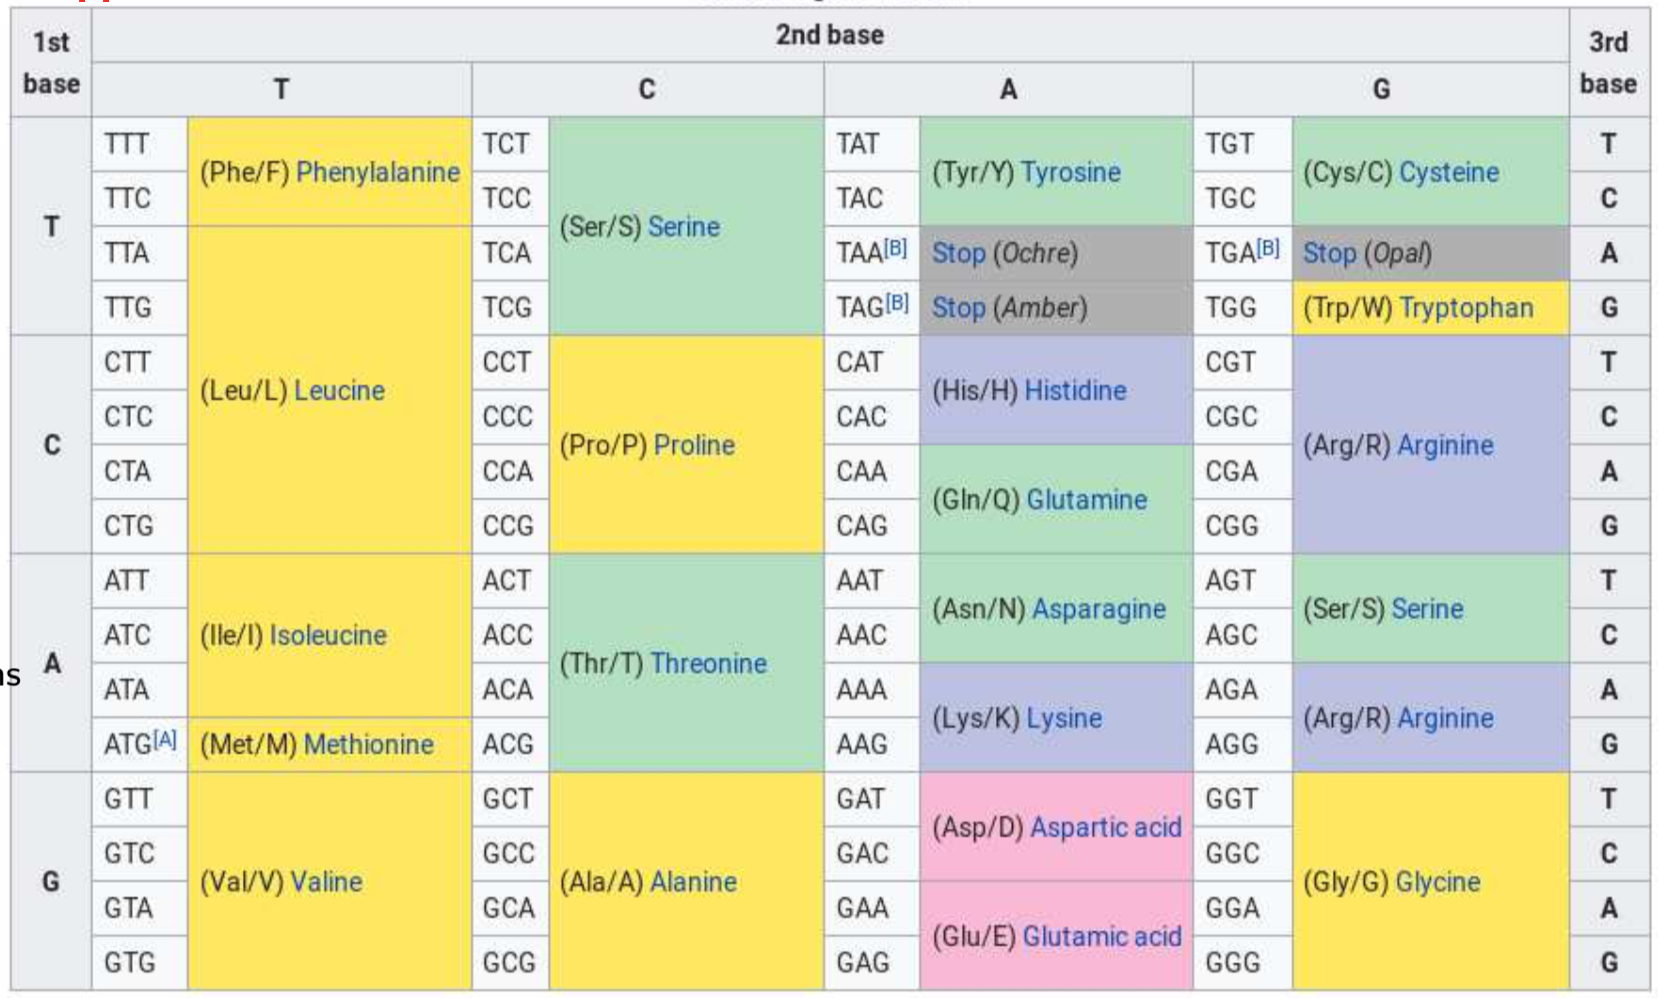
\includegraphics[width=400px]{images/2.3_codons-aminoacids}

\emph{Saving the nucleotide sequence from GenBank:}

The complete nucleotide sequence of the coding strand from GenBank
(\url{https://www.ncbi.nlm.nih.gov/nuccore/CU329670.1?from=1\&to=5662})
was saved in FASTA format as \textbf{2.3\_nucleotid-sequence.FASTA}.
Note that only the last 12 characters AGCGACGACCAT actually correspond
to the amino acids MVVA if the reverse compliment is taken (see 2.4).

\emph{Using backtrack to obtain the amino acid sequence from the protein
sequence:}

We used backtrack to obtain the amino acid sequence corresponding to the
protein sequence \texttt{MVVA}
(\url{https://www.ebi.ac.uk/Tools/st/emboss_backtranseq/}). After
pasting \texttt{MVVA} and selecting ``Schizosaccharomyces pombe (CAI
equivalent)'', the following sequence is returned: \textbf{ATGGTCGTCGCT}

\subsection{2.4}\label{section-3}

The above mentioned obtained coding strand sequence ATGGTCGTCGCT does
not exist in the provided nucleotide sequence (that was saved in FASTA
format as 2.3\_nucleotid-sequence.FASTA) since this sequence is not
found when searching the file.

\emph{Option 1}

However, we can modify the displayed sequence to get what we are looking
for. On GenBank, under ``Display options'', one has to select both
``Show sequence'' and \textbf{``Show reverse complement''}
(\url{https://www.ncbi.nlm.nih.gov/nuccore/CU329670.1?from=1\&to=5662}).
Afterwards, the displayed nucleotid sequence under ``ORIGIN'' starts
with ATGGTCGTCGCT which codes for our amino acids MVVA.

\emph{Option 2}

Alternatively, one can take the last 12 characters from the original
nucleotid sequence (the one in the FASTA file, i.e.~the sequence before
selecting ``Show reverse complement'' on GenBank). These characters are:
AGCGACGACCAT. Copy this string and paste it here:
\url{http://arep.med.harvard.edu/labgc/adnan/projects/Utilities/revcomp.html}
Then click \textbf{``reverse complement''}. The result is again the
sequence that we are looking for: ATGGTCGTCGCT which codes for our amino
acids MVVA.

\emph{Conclusion}

\textbf{ATGGTCGTCGCT is exactly what we got in 2.3 using backtranseq} to
obtain the amino acid sequence from the protein sequence \texttt{MVVA}.
The only tricky thing here was that we needed to take the reverse
complement of the correct characters from the nucleotid sequence (namely
the last 12 characters).

\subsection{2.5}\label{section-4}

\emph{Number range that corresponds to these amino acids (protein
sequence):}

In the saved FASTA file, the \emph{last 12 characters} AGCGACGACCAT
correspond to the amino acids MVVA (after taking the reverse
complement). The number range corresponding to them is 5651 to 5662.

If we had selected ``Show reverse complement'' on GenBank before, then
the \emph{first 12 characters} ATGGTCGTCGCT would correspond to the
amino acids MVVA. The number range would then be 1 to 12.

\emph{Stop codon in the nucleotide sequence:}

Note that there are three possible stop codons: TAA, TAG, TGA. Still, it
is not easy to identify the stop codon manually. However, one can use:
\url{https://www.ncbi.nlm.nih.gov/orffinder} and paste the complete
(reverse complement) nucleotide sequence in FASTA format. With the
default parameters, this is automatically translated to the correct
amino acid sequence. Also, after scolling down a bit, one can see that
the last stop happens at 5661. We find TC from 5661 to 5662 (and at
5662, we have the last nucleotid). From 5658 to 5660, we have TGA which
is one of the above mentioned stop codons. We can conclude that the stop
codon in the nucleotid sequence is hence TGA from 5658 to 5660 (looking
at the reverse complement nucleotid sequence).

\emph{Chromosome on which the genomic sequence lies:}

We can see on GenBank (in the header under the definition as well as in
the features under source), that this genomic sequence lies on the
chromosome 1 of schizosaccharomyces pombe.

\section{Assignment 3}\label{assignment-3}

\subsection{3.1}\label{section-5}

Caenorhabditis elegans is a free-living, nematode worm, which lives in
soil environments all over the world. it is divided in two sexes:

\begin{enumerate}
\def\labelenumi{\roman{enumi})}
\tightlist
\item
  male
\item
  self-fertilizing hermaphrodite
\end{enumerate}

Finally, it has all human sensations, such as taste and smell, despite
the fact that is has no eyes.
(\url{https://en.wikipedia.org/wiki/Caenorhabditis_elegans})

In general C.elegans has a similar construction and characteristics as
humans. It is also important that the genes, which are responsible for
human's evolution, had similar ancestor with C.elegans. Therefore,
instead of making experiments on humans, which most of the time is
expensive and difficult, scientist can work with C.elegans. That is the
reason why studying C.elegans biology is crucial for scientific field.
(\url{http://www.people.ku.edu/~erikl/Lundquist_Lab/Why_study_C._elegans.html})

\subsection{3.2}\label{section-6}

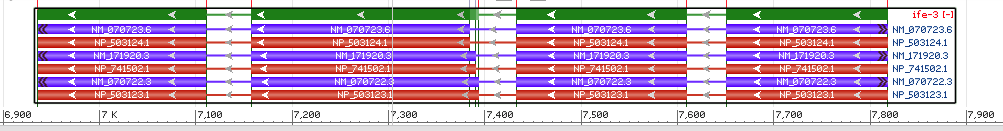
\includegraphics[width=18.86in]{images/3.2_exons}

This diagram shows exons and introns. We have 4 exons in our searching
query. Our searching query found between 6528 and 8027. Our exons and
introns:\\
* introns1: 6528 - 6935 * exon1: 6936 - 7110 * introns2: 7111 - 7157 *
exon2: 7158 - 7393 * introns3: 7394 - 7432 * exon3: 7433 - 7609 *
introns4: 7610 - 7650 * exon4: 7651 - 7818 * introns5: 7819 - 8027

\section{Appendix}\label{appendix}

\begin{Shaded}
\begin{Highlighting}[]
\NormalTok{knitr}\OperatorTok{::}\NormalTok{opts_chunk}\OperatorTok{$}\KeywordTok{set}\NormalTok{(}\DataTypeTok{fig.width =} \DecValTok{7}\NormalTok{, }\DataTypeTok{fig.height =} \DecValTok{3}\NormalTok{, }\DataTypeTok{echo =} \OtherTok{FALSE}\NormalTok{) }

\KeywordTok{library}\NormalTok{(dplyr)}
\KeywordTok{library}\NormalTok{(tidyr)}
\KeywordTok{library}\NormalTok{(magrittr)}
\KeywordTok{library}\NormalTok{(kableExtra)}

\CommentTok{# ------------------------------------------------------------------------------}
\CommentTok{# Question 1.2}
\CommentTok{# ------------------------------------------------------------------------------}

\CommentTok{# The prob of one allele is the proportion of the homozigote + half the proportion of the heterozygote }
\NormalTok{p =}\StringTok{ }\FloatTok{0.357} \OperatorTok{+}\StringTok{ }\FloatTok{0.485} \OperatorTok{/}\StringTok{ }\DecValTok{2}
\NormalTok{q =}\StringTok{ }\FloatTok{0.158} \OperatorTok{+}\StringTok{ }\FloatTok{0.485} \OperatorTok{/}\StringTok{ }\DecValTok{2}

\CommentTok{# Expected values (Hardy–Weinberg equilibrium)}
\NormalTok{p_}\DecValTok{2}\NormalTok{ =}\StringTok{ }\NormalTok{p}\OperatorTok{^}\DecValTok{2}
\NormalTok{q_}\DecValTok{2}\NormalTok{ =}\StringTok{ }\NormalTok{q}\OperatorTok{^}\DecValTok{2}
\NormalTok{pq =}\StringTok{ }\DecValTok{2}\OperatorTok{*}\NormalTok{p}\OperatorTok{*}\NormalTok{q}

\NormalTok{Xsq =}\StringTok{ }\KeywordTok{chisq.test}\NormalTok{(}\KeywordTok{c}\NormalTok{(}\FloatTok{0.357}\NormalTok{, }\FloatTok{0.485}\NormalTok{, }\FloatTok{0.158}\NormalTok{), }\DataTypeTok{p=}\KeywordTok{c}\NormalTok{(p_}\DecValTok{2}\NormalTok{, pq, q_}\DecValTok{2}\NormalTok{))}
\NormalTok{Xsq}
\CommentTok{# Xsq$observed}
\CommentTok{# Xsq$expected}

\NormalTok{knitr}\OperatorTok{::}\KeywordTok{include_graphics}\NormalTok{(}\StringTok{"images/2.2_amino-acids.png"}\NormalTok{)}
\NormalTok{knitr}\OperatorTok{::}\KeywordTok{include_graphics}\NormalTok{(}\StringTok{"images/2.3_nucleotides.png"}\NormalTok{)}
\NormalTok{knitr}\OperatorTok{::}\KeywordTok{include_graphics}\NormalTok{(}\StringTok{"images/2.3_codons-aminoacids"}\NormalTok{)}
\CommentTok{# ------------------------------------------------------------------------------}
\CommentTok{# Question 3.2}
\CommentTok{# ------------------------------------------------------------------------------}
\NormalTok{knitr}\OperatorTok{::}\KeywordTok{include_graphics}\NormalTok{(}\StringTok{"images/3.2_exons.png"}\NormalTok{)}
\end{Highlighting}
\end{Shaded}


\end{document}
